%----------------------------------------------------------------------------------------
%	SECTION 1
%----------------------------------------------------------------------------------------

\section{The Rank of a Matroid.}

Let $M=(E,\Ic)$ be a matroid, and let $X \subseteq E$, and  $\Ic|X=\{I \subseteq
X : I \in \Ic\}$. Then the pair $(X,\Ic|X)$ forms a matroid which we can define
as follows.

\begin{definition}
    If $M=(E,\Ic)$ is a matroid, and $X \subseteq E$, then we call the matroid
    $M|X=(X,\Ic|X)$ the \textbf{restriction} of $M$ to  $X$, or alternatively,
    the \textbf{deletion} of $\com{E}{X}$ from $M$.
\end{definition}

This also motivates the following definition for the ``rank'' of a matroid.

\begin{definition}
    Let $M=(E,\Ic)$ bea matroid, and $X \subseteq E$. We define the
    \textbf{rank} of $X$ to be the cardinality of some basis  $B$ of  $M|X$, and
    denote it  $\rank{X}$; we also call $B$ a  \textbf{basis} of $X$. We define
    the  \textbf{rank function} of the matroid $M$ to be the mapping  $\rank:2^E
    \rightarrow \N$, and we write $\rank{M}=\rank{E}$. That is the rank of the
    matroid $M$ is the rank of its ground set.
\end{definition}

\begin{lemma}\label{1.3.1}
    Let $M$ be a matroid on a set  $E$, and let $X \subseteq E$. If $\rank$ is
    the rank function of  $M$, then the following are true:
    \begin{enumerate}
        \item[(R1)] $0 \leq \rank{X} \leq |X|$.

        \item[(R2)] If  $Y \subseteq E$ with  $X \subseteq Y$, then  $\rank{X}
            \leq \rank{Y}$.

        \item[(R3)] If $X \subseteq E$ and  $Y \subseteq E$, then $\rank{(X \cup
            Y)}+\rank{(X \cap Y)} \leq \rank{X}+\rank{Y}$.
    \end{enumerate}
\end{lemma}
\begin{proof}
    Since $\rank$ maps a subset of $E$ to a nonnegative integer in $\N$, we see
    that  $\rank{X} \geq 0$. Now, if $B$ is a basis of $X$, then  $B \subseteq
    X$, so that  $|B| \leq |X|$, so  $\rank{X} \leq |X|$.

    Moreover, if $X \subseteq Y$, and  $B$ is a basis
    of  $X$, then it is a basis of the matroid  $M|X$, as well as being an
    independent set of the matroid $M|Y$. So if  $B'$ is the basis for  $Y$;
    i.e. a basis of  $M|Y$, then we have  $|B| \leq |B'| \leq |Y|$, so that
    $\rank{X} \leq \rank{Y}$

    Now, let $B_{X \cap Y}$ be a basis of $X \cap Y$, then it is an independent
    set in  $M|(X \cup Y)$, and hence contained in a basis $B_{X \cup Y}$ of $X
    \cup Y$. Now, we also have that  $B_{X \cup Y} \cap X$ and $B_{X \cup Y}
    \cap Y$ are independent in  $M|X$ and  $M|Y$, respectively; So we get that
    $\rank{X} \geq |B_{X \cup Y} \cap X|$ and $\rank{Y} \geq |B_{X \cup Y} \cap
    Y|$, thus $\rank{X}+\rank{Y} \geq |B_{X \cup Y} \cap X|+|B_{X \cup Y} \cap
    y|=|B_{X \cup Y}|+|B_{X \cap Y}|=\rank{(X \cup Y)}+\rank{(X \cap Y)}$.
\end{proof}
\begin{corollary}
    For any matroid $M$ on  $E$ with $X \subseteq E$ and  $x \in E$:
    \begin{equation*}
        \rank{X} \leq \rank{(X \cup x)} \leq \rank{X}+1
    \end{equation*}
\end{corollary}

\begin{example}\label{1.11}
    \begin{enumerate}
        \item[(1)] Let $V$ be a vector space and consider the matroid $M[V]$ on
            $V$, the dimension of $V$ is a rank function of $M[V]$ by definition.
            Moreover, if $U$ and  $W$ are subspaces of  $V$, then we can define
            matroids  $M[U]$ and $M[W]$ on $U$ and  $W$, respectively by taking
            $M[U]=M[V]|U$ and $M[U]=M[W]|W$, morevoer, we also get by a well
            known theorem of linear algebra that
                \begin{equation*}
                    \dim{(U+W)}+\dim{(U \cap W)}=\dim{U}+\dim{W}
                \end{equation*}

            \item[(2)] Infact, for any representable matroid $M[V]$ over a
                vector space $V$, by above we get that (R3) attains equality, so
                that any matroid isomorphic to $M[V]$ attains equality on (R3).

            \item[(3)] Let $M$ be a matroid, and let  $B_X$ be a basis of $X$ in
                $M$, now suppose that  $I \subseteq \com{E}{X}$ such that
                $I \cup B$ is independent. Then by definition of independence
                via the rank, we have $\rank{(I \cup B)}=|I \cup B|=|I|+|B|$.
                Now suppose $X' \subseteq X$ is also independent, then
                $\rank{X'}=|X'|$. Then $B$ is a basis of  $X$, so  $|X'| \leq
                |B|$, so we can take the complement of  $B$ with respect to
                $X'$. Now since $B$ is independent, we must also have that
                $\com{B}{X} \subseteq B$ must also be independent, so we get that
                $\rank{(\com{B}{X'})}=|B|-|x'|$, then we have that
                $\rank{(I \cup B)}-\rank{(\com{B}{X'})}=|I|+|B|-|B|+|X'|=|I|+|X'|
                =|I \cup X'|$. Moreover, $\rank{(\com{(I \cup
                B)}{(\com{B}{X'})})}=\rank{(I \cup X')}=|I \cup X'|$. This makes
                $I \cup X'$ independent as well.

    \end{enumerate}
\end{example}

\begin{lemma}\label{1.3.2}
    Let $E$ be a set and  $r:2^E \rightarrow \N$ be a mapping satisfying (R1)
    and (R2). if $X$ and  $Y$ are subsets of  $E$ such that  $r(X \cup y)=r(X)$
    for all $y \in \com{Y}{X}$, then $r(X \cup Y)=r(X)$.
\end{lemma}
\begin{proof}
    Let $\com{X}{Y}=\{y_1, \dots, y_n\}$. Then by induction on $n$, when  $n=1$,
    we have by hypothesis thay  $r(X \cup y_1)=r(X)$. Now suppose thta $r(X \cup
    \{y_1, \dots y_n\})=r(X)$ for all $n \geq 1$, and consider the set
    $\{y_1,\dots,y_{n+1}\}$. Then we get that
    \begin{align*}
        r(X)+r(X)   &=  r(X \cup \{y_1, \dots, y_n\})+r(X \cup y_{n+1}) \\
                    & \geq r(X \cup \{y_1, \dots y_{n+1}\})+r(X \cap \{y_1,
                        \dots y_{n+1}\}) \\
                    &= r(X \cup \{y_1, \dots y_{n+1}\})+r(X) \\
                    & \geq r(X)+r(X)
    \end{align*}
    So by equality, we get that $r(X \cup \{y_1, \dots, y_{n+1}\})=r(X)$.
\end{proof}

\begin{theorem}\label{1.3.3}
    Let $E$ be a set and $r:2^E \rightarrow \N$ be a mapping of $2^E$ into
    $\N$ such that $r$ satisfies (R1)-(R3). If $\Ic=\{X \subseteq E :
    r(X)=|X|\}$ Then $r$ is the rank function of a matroid $M$ on $E$
\end{theorem}
\begin{proof}
    By (R1), we havbe that $0 \leq r(\emptyset) \leq |\emptyset|=0$, so
    $r(\emptyset)=|\emptyset|=0$; this makes $\emptyset \in \Ic$.

    Now, suppose that $I \in \Ic$ and that  $\Ic' \subseteq I$. Then
    $r(I)=|I|$, and $r(I' \cup (\com{I}{I'}))+r(I' \cap (\com{I}{I'})) \leq
    r(I')+r(\com{I}{I'})$, so $r(I) \leq r(I')+r(\com{I}{I'})$, i.e. $|I| \leq
    r(I')+r(\com{I}{I'}) \leq |I'|+|\com{I}{I'}|=|I|$. This makes $r(I')=|I'|$,
    so that $I' \in \Ic$.

    Now suppose that $I,I' \in \Ic$, with  $|I|<|I'|$, and suppose for all $e
    \in \com{I'}{I}$ that $I \cup e \notin \Ic$, that is  $r(I \cup e) \neq |I
    \cup e|=|I|+1$. Now, we have that $|I|=r(I) \leq r(I \cup e)<|I|+1$, so $r(U
    \cup e)=r(I)=|I|$; then by lemma \ref{1.3.2}, we have $r(I \cup I')=r(I)$,
    but we also have that $r(I \cup I') \geq r(I')=|I'|$ making $|I| \geq |I'|$,
    a contradiciton, therefore  $I \cup e \in \Ic$ for all  $e \in \com{I'}{I}$.
    This makes $M$ into a matroid on $E$.

    Now suppose that $X \in \Ic$ is independent. Then  $r(X)=|X|$, moreover, $X$
    is a basis for the matroid  $M|X$, so that  $r(X)=\rank{X}$. Now if $X$
    isn't independent, and  $B$ is a basis for  $M|X$, then we have
    $\rank{B}=|B|$, moreover, $B \cup x \notin \Ic$ for any  $x \in \com{X}{B}$,
    so that $|B|=r(B) \leq r(B \cup x)<|B \cup x|$, making $r(B \cup x)=r(B)$.
    This makes $r(X)=r(B)=|B|=\rank{X}$, therefore $r=\rank$, and  $r$ is the
    rank function on  $M$.
\end{proof}
\begin{corollary}
    $r$ is the rank function of a matroid on  $E$ if, and only if it satisfies
    (R1)-(R3).
\end{corollary}

This gives the next definition of a matroid.

\begin{definition}
    A \textbf{matroid} on a finite nonempty set $E$ is a pair  $M=(E,\rank)$
    where $\rank:2^E \rightarrow \N$ is a mapping taking subsets of $E$ to  $\N$
    such that:
    \begin{enumerate}
        \item[(R1)] $0 \leq \rank{X} \leq |X|$ for all $X \subseteq E$

        \item[(R2)] If $X \subseteq Y \subseteq E$, then  $\rank{X} \leq
            \rank{Y}$.
        \item[(R3)] If $X,Y \subseteq E$, then  $\rank{X \cup Y}+\rank{X \cap Y}
            \leq \rank{X} + \rank{Y}$.
    \end{enumerate}
    We call $\rank{X}$ the \textbf{rank} of $X$, and we call  $\rank$ the
    \textbf{rank function} of the matroid $M$.
\end{definition}

\begin{theorem}\label{1.3.4}
    Let $M$ be a matroid on a set  $E$ together with a rank function  $\rank$.
    Then the following are true for any $X \subseteq E$:
    \begin{enumerate}
        \item[(1)] $X$ is independent if, and only if  $\rank{X}=|X|$.

        \item[(2)] $X$ is a basis if, and only if  $\rank{X}=\rank{M}$.

        \item[(3)] $X$ is a circuit if, and only if  $X$ is nonempty and for all
             $x \in X$,  $\rank{(\com{X}{x})}=|X|-1=\rank{X}$.
    \end{enumerate}
\end{theorem}
\begin{proof}
    The first statement follows immediately from theorem \ref{1.3.3}. Now,
    suppose that $X$ is a basis of the matroid $M$, then $X$ is independent, so
     $\rank{X}=|X|$, and by definition $\rank{M}=|X|$. Conversely, if $X
     \subseteq E$ such that  $\rank{M}=\rank{X}$, then by definition
     $\rank{M}=|B|$ for some basis $B$ of  $M$, and $|B|=\rank{X}$, this makes
     $X$ an independent set, then by the first statement,  $\rank{X}=|X|=|B|$,
     making $X$ a basis.

     Now, suppose that $X$ is a circuit, then by minimality, $\com{X}{x}$ is
     independent whenever $x \in X$, so that
     $\rank{(\com{X}{x})}=|\com{X}{x}|=|X|-1=\rank{X}$. Conversely, suppose for
     $X$ nonempty that  $\rank{(\com{X}{x})}=|X|-1=\rank{X}$ whenever $x \in X$.
     Then we have that since $\rank{(\com{X}{x})}=|X|-1=|\com{X}{x}|$,
     $\com{X}{x}$ is independent, but since $\rank{X}=|X|-1$, $X$ is not
     independent. That makes  $X$ a minimally dependent set of $E$, thus $X$ is
     a circuit of $M$.
\end{proof}

\begin{example}\label{1.12}
    \begin{enumerate}
        \item[(1)] Let $E$ be any set, and consider the uniform matroid
            $U_{m,n}$ for $m,n \in \Z^+$. Then by definition, the rank function
            of  $U_{m,n}$ is defined to be:
            \begin{equation*}
                \rank{X}=\begin{cases}
                            |X|, \text{ if } |X|<m \\
                            m, \text{ if } |X| \geq m \\
                         \end{cases}
            \end{equation*}

            In fact, any matroid is isomorphic to a uniform matroid if and only
            if there are no circuits of size less than $\rank{M}+1$. By
            definition, we have that if $U_{m,n}$ is the uniform matroid of
            rank $m$, then by definition the circuits are those sets  $C$ for
            which  $|C|=m+1$; so any matroid isomorphic to  $U_{m,n}$ must also
            satisfy this. Conversely, if $M$ is a matroid of rank $m$, with all
            circuits $C$ of size $m+1$, then by minimality of $C$,
            $I=\com{C}{c}$ is maximally independent for appending any element
            makes it of size $m+1$, which necesarily makes it a circuit. Thus
            $I$ is a base, so that $\rank{I}=m$, since $C$ is arbitrary, so is
            $I$, this then makes  $M$ isomorphic to $U_{m,n}$.

            It happens for $U_{1,n}$, (R3) does not attain equality. Notice any
            basis $B$ has  $\rank{B}=1$, and any circuit $C$ has
            $\rank{C}=1$, so $\rank{B}+\rank{C}=2$. However, if $B$ and $C$ are
            disjoint, then  $\rank{(B \cup C)}=1$ and $\rank{(B \cap C)}=0$, so
            that $\rank{(B \cup C)}+\rank{(B \cap C)}=1<2$.

        \item[(2)] If $A$ is an  $m \times n$ matrix over a field  $F$, then the
        rank function of  $M[A]$ is the rank of the $m \times |X|$ submatrix
        $A|X$ consisting of columns of $A$ labeled by members of $X$. Moreover,
        the rank of $X$ is the dimension of the subspace of the vector space
        over  $F$ spanned by the columns of  $A|X$.

    \item[(3)] Let $G$ be a graph and $M(G)$ be the graphic matroid on $G$. If
        $G$ is conneced, then a basis of  $G$ is a spanning tree  $T$ of  $G$,
        for which  $|V(T)|=|E(T)|+1$, so the rank of $M(G)$ in this case is:
        \begin{equation*}
            \rank{M(G)}=|V(G)|-1
        \end{equation*}
        Now, if $G$ has  $\omega$ connected components, then by similar
        reasoning, the rank of  $M(G)$ is:
        \begin{equation*}
            \rank{M(G)}=|V(G)|-\omega
        \end{equation*}
        Now, if $X$ is a subset of edges of  $G$, then
        \begin{equation*}
            \rank{X}=|V(X)|-\omega_X
        \end{equation*}
        where  $\omega_X$ is the number of connected components of  $X$.

    \item[(4)]
         \begin{figure}[h]
            \centering
            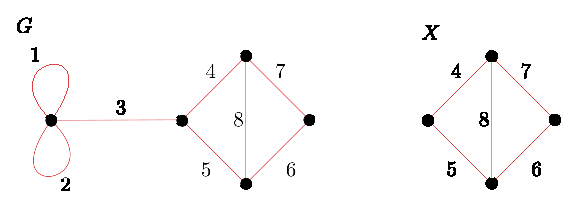
\includegraphics[scale=1.0]{Figures/Chapter1/connected_graph_rank.eps}
            \caption{}
            \label{fig_1.6}
        \end{figure}
        Let $G$ be the graph in figure \ref{fig_1.6}, then $G$ is a connected
        graph so  $\rank{M(G)}=|V(G)|-1=4$. Now, if $X=\{4,5,6,7,8\}$, then
        $M(X)=M(G)|X$ has as a basis the set $\{4,7,8\}$, so that $\rank{X}=3$.
        If $Z=\{1,2\}$, then $M(Z)$ only has $\emptyset$ as a basis, so that
        $\rank{Z}=0$.

    \item[(5)] In any matroid $M$, we have an element $x$ is a loop if, and only
        if  $\rank{\{x\}}=0$, and two elements $x$ and $y$ are parallel if and
        only if $\rank{\{x,y\}}=1$.

        Certainly, if $x$ is a loop, then  $\{x\}$ is a circuit, so that the
        only basis of $M|\{x\}$ is $\emptyset$, this makes  $\rank{\{x\}}=0$.
        Likewise, if $x$ and  $y$ are parallel, then $\{x,y\}$ is a circuit,
        making $\{x\}$ and $\{y\}$ maximally independnet, and hence bases of
        $M|\{x,y\}$, thus $\rank{\{x,y\}}=1$.

        Conversely, if $\rank{\{x\}}$, then $\{x\}$ only has $\emptyset$ as a
        basis, hence $\{x\}$ is minimally dependent, hence a circuit, hence it
        is a loop. By similar reasoning for parallel elements, if
        $\rank{\{x,y\}}=1$, then $x || y$.
    \end{enumerate}
\end{example}

\begin{lemma}\label{1.3.5}
    Let $M$ be a matroid and  $k \in \N$ such that  $k \leq \rank{M}$. Define
    the map $r_{(k)}:2^E \rightarrow \N$ by $r_{(k)}(X)=\min{\{k,\rank{X}\}}$.
    Then $r_{(k)}$ is the rank function for a matroid.
\end{lemma}
\begin{proof}
    Certainly by definition, we have $0 \leq r_{(k)}(X) \leq |X|$. Moreover, if
    $X \subseteq Y$, then  $\min\{k,\rank{X}\} \leq \min\{k,\rank{Y}\}$, so we get
    $r_{(k)}(X) \leq r_{(k)}(Y)$.

    Now, if $X$ and  $Y$, then we get $r_{(k)}(X \cup Y)=\min\{k,\rank{(X \cup
    Y)}\}$, and $r_{(k)}(X \cap Y)=\min\{l, \rank{(X \cap Y)}\}$, then
    $r_{(k)}(X \cup Y)+r_{(k)}(X \cap Y)=\min\{k, \rank{(X \cup Y)}+\rank{X \cap
    Y}\} \leq \min\{k, \rank{X}+\rank{Y}\}=r_{(k)}(X)+r_{(k)}(Y)$. This makes
    $r_{(k)}$ the rank function of the matroid.
\end{proof}
\begin{corollary}
    $r_{(k)}(M)=k$
\end{corollary}
\begin{proof}
    We have that $k \leq M$, so  $r_{(k)}(M)=\min\{k,\rank{M}\}=k$ in all cases.
\end{proof}
\begin{remark}
    We call this matroid obtained through $r_{(k)}$ a matroid obtained by a
    sequence of ``truncations'' . The collection of independent sets on these
    matroids are the collection of all independent sets of $M$ of size less than
    or equal to  $k$. That is:
    \begin{equation*}
        \Ic=\{I \subseteq M : |I| \leq k\}
    \end{equation*}
\end{remark}

\begin{definition}
    We call a matroid \textbf{paving} if it has no circuits of size less than
    $\rank{M}$.
\end{definition}

\begin{example}\label{1.13}
    For any $m,n \in \Z^+$, the uniform matroid  $U_{m,n}$ only has circuits of
    size $m+1$, thus  $U_{m,n}$ is paving for all $m,n \in \Z^+$. In general, a
    matroid has circuits of size at most  $\rank{M}+1$, so that $M$ is uniform
    if, and only if it has no circuits of size less than $\rank{M}+1$. So a
    useful check for determining whether a matroid is paving is to show that it
    is uniform. However, not every paving matroid is uniform. For example, the
    matroid $M(K_5)$ on the complete graph on $5$ vertices is paving, but not
    uniform.
\end{example}

\begin{theorem}\label{1.3.6}
    Let $\Dc$ bea collection of nonempty subsets of a set $E$. Then  $\Dc$ is
    the collection of circuits of a paving matroid on  $E$ if, and only if there
    is a  $k \in \Z^+$ with  $k<|E|$, and a subcollection  $\Dc' \subseteq \Dc$
    such that:
    \begin{enumerate}
        \item[(1)] Every $D' \in \Dc'$ has  $k$ elements and if  $D',D'' \in
            \Dc'$ are distinct, then ${D' \cup D'' \choose k} \in \Dc'$.

        \item[(2)] $\com{\Dc}{\Dc'}$ consists of all $k+1$-element subsets
            containing no member of  $\Dc'$.
    \end{enumerate}
\end{theorem}

\begin{lemma}[Brylawski]\label{1.3.6}
    Let $M$ be a matroid on a set  $E$, and let  $k \in \N$ such that  $\rank{M}
    \leq k \leq |E|$. Then if $S_k$ is the collection of all  $k$-element
    subsets of  $E$ with rank  $\rank{M}$, then $S_k$ is the collection of basis
    of a matroid on $E$.
\end{lemma}
\begin{proof}
    Notice by definition that if $S,S' \in S_k$, then  $|S|=|S'|$. Now, if
    $S_k$ is empty that means no  $k$-element suibset of  $E$ has rank
    $\rank{M}$, then if $k=|E|$,  $\rank{E} \neq \rank{M}$, which cannot happen.
    So we have that $S_k$ is nonempty.

    Now let  $S,S' \in S_k$, then  $ \rank{S}=\rank{S'}=\rank{M}$. Now choose $s
    \in \com{S}{S'}$, then $\com{S}{s}$ is a $k-1$-element set. Taking $s' \in
    \com{S'}{S}$, we have $(\com{S}{s}) \cup s'$ is a $k$-element subset of
    $E$, hence $|(\com{S}{s}) \cup s'| \leq |E|$  so we get $\rank{(\com{S}{s})
    \cup s'} \leq \rank{E}=\rank{M}$, moreover, we have that $\rank{S} \leq
    \rank{((\com{S}{s}) \cup s')}$ by the corollary to lemma \ref{1.3.1}, so we
    get that $\rank{(\com{S}{s}) \cup s'}=\rank{S}=\rank{M}$, which makes
    $(\com{S}{s}) \cup s' \in S_k$. This makes $S_k$ the collection of bases of
    a matroid on  $E$.
\end{proof}

\begin{definition}
    Let $M$ be a matroid on  $E$, we define the  \textbf{elongation} of $M$ to
    rank  $k$, where  $\rank{M} \leq k \leq |E|$ to be the matroid on $E$ having
    collection of bases $S_k$ the collection of all $k$-element subsets of  $E$
    of \rank{M}. If $k=\rank{M}+1$, we call the elongation of $M$ the
    \textbf{Higgs lift} of $M$.
\end{definition}

\begin{lemma}[Edmonds and Rota]\label{1.3.8}
    Let $f:2^E \rightarrow \N$ be a mapping of subsets of a set $E$ satisfying
    the following:
    \begin{enumerate}
        \item[(1)] $f(\emptyset)=0$.

        \item[(2)] If $X \subseteq Y$, then  $f(X) \leq f(Y)$.

        \item[(3)] $f(X \cup Y)+f(X \cap Y) \leq f(X)+f(Y)$.
    \end{enumerate}
    Then $f$ defines a matroid  $M$ on  $E$  having the collection of
    independent sets  $\Ic(f)=\{X \subseteq E : f(X) \geq |X|\}$.
\end{lemma}
\begin{proof}
    By definition, we have $f(\emptyset)=0=|\emptyset|$, so $\emptyset \in
    \Ic(f)$. Now, suppose that $Y \in \Ic(f)$, then $f(Y) \geq |Y|$, now if $X
    \subseteq Y$, we either have $|X| \leq f(X) \leq |Y| \leq f(Y)$, or $|X|
    \leq |Y| \leq f(X) \leq f(Y)$; either case inheretence is satisfied, and $X
    \in \Ic(f)$.

    Now suppose that $X,Y \in \Ic(f)$, and that $|X|<|Y|$. Now, let $y \in
    \com{Y}{X}$, and suppose that $f(X \cup y)<|X \cup y|=|X|+1$,
    then we have $f(X \cup y) \leq f(X)+f(y)-f(X \cap y)=f(X)+f(y) \leq |X|+1
    \leq f(X)+f(y)$, which makes $f(X)=|X|$ and $f(y)=1$, thus we get $f(X \cup
    y)=f(X) + f(y)=|X|+1$, which contradicts the assumption. Thus we must have
    that $|X \cup e| \leq f(X \cup e)$. This makes $X \cup e \in \Ic(f)$, and
    makes $\Ic(f)$ the collection of independent sets of a matroid on $E$.
\end{proof}
\begin{corollary}
    The rank function of the matroid $M=(E,\Ic(f))$ is the map $r:2^E
    \rightarrow \N$ defined by:
        \begin{equation*}
            r(X)=\begin{cases}
                    |X|, \text{ if } f(X)=|X| \\
                    |B|, \text{ for some } B \subseteq X \text{ such that }
                    f(B)=|B| \\
                 \end{cases}
        \end{equation*}
\end{corollary}
\begin{proof}
    Let $X \in \Ic(f)$ be independent. Then we see that $f(X) \geq |X|$. Then
    $X$ is dependent if  $f(X)<|X|$. Thus, $X$ is a basis if, and only if
    $f(X)=|X|$.
\end{proof}
\begin{remark}
    We call mappings satisfying properties (1)-(3) of lemma \ref{1.3.8}
    \textbf{submodular functions}, and we will study them and their matroids
    later on. It is no surprise that the rank function is also a submodular
    function.
\end{remark}
